\documentclass[a4paper]{article}

%% Language and font encodings
\usepackage[english]{babel}
\usepackage[utf8x]{inputenc}
\usepackage[T1]{fontenc}
\usepackage{float}


%% Sets page size and margins
\usepackage[a4paper,top=.5cm,bottom=.5cm,left=3cm,right=3cm,marginparwidth=1.75cm]{geometry}

%% Useful packages
\usepackage{amsmath}
\usepackage{graphicx}
\usepackage[colorinlistoftodos]{todonotes}
\usepackage[colorlinks=true, allcolors=blue]{hyperref}

\title{3I005 Projet Classification d'Emails}
\author{BEROUKHIM Keyvan MONGENOT Nicolas}
\date{}

\begin{document}
\maketitle

\section{Introduction}
De nombreuses boîtes de messagerie proposent des services de tri des e-mails, tels que le tri par contact, par date, etc … De même, ces messageries détectent les spams et les placent dans un dossier « indésirables ».
Dans ce TME, nous allons essayer de comprendre comment fonctionne une technique de détection des spams et de quels facteurs elle dépend. \\
Dans un premier temps, nous allons supposer que seule la taille permet de détecter si un mail est ou non un spam.\\
Nous verrons que la taille n’est pas un argument suffisamment précis pour dire qu’un e-mail est un spam, le taux d’erreur étant très élevé.
Puis dans un second temps, nous regarderons le contenu des e-mails pour tenter de les classifier, c’est-à-dire qu’en fonction des mots utilisés, nous pourrons prédire si cet e-mail est un spam.\\
Nous avons utilisé les bases de mails fournies.
\section{Classification à partir de la longueur d'un e-mail}
\subsection{} \label{partie2.1}

P(Y = 1 | X = x): probabilité que le mail soit du spam sachant qu'il a une taille de x mots.\\
P(X = x | Y = 1): probabilité que le mail fasse x mots de long sachant que c'est du spam.\\
P(Y = 1): probabilité que le mail soit du spam.\\
P(X = x): probabilité que le mail ait une taille de x mots.\\\\
Étant donné un mail, on peut mesurer sa longueur X. On cherche à déterminer si c'est du spam ou non. L'objectif est donc de comparer P(Y = 1 | X = x) et P(Y = -1 | X = x).
Or, on a :
$$P(Y = 1 | X = x) = P(X = x | Y = 1) * P(Y = 1) / P(X = x)$$ et
$$P(Y = -1 | X = x) = P(X = x | Y = -1) * P(Y = -1) / P(X = x)$$
De plus, on considère que
$$P(Y = 1) = P(Y = -1) = 50\%$$ 
On peut alors simplifier :
$$P(Y = 1 | X = x) > P(Y = -1 | X = x)	\Leftrightarrow P(X = x | Y = 1) > P(X = x | Y = -1)$$
\\
A partir d'un ensemble de mails connus comme spam, on peut estimer la distribution P(X=x|Y=1) en mesurant la distribution des tailles. De même pour P(X=x|Y=-1) à partir d'un  ensemble de mails connus comme n'étant pas du spam.\\
Il n'est donc pas nécessaire de calculer P(X = x) ou P(Y = 1).

\subsection{}
\begin{minipage}{\textwidth}
\begin{figure}[H]
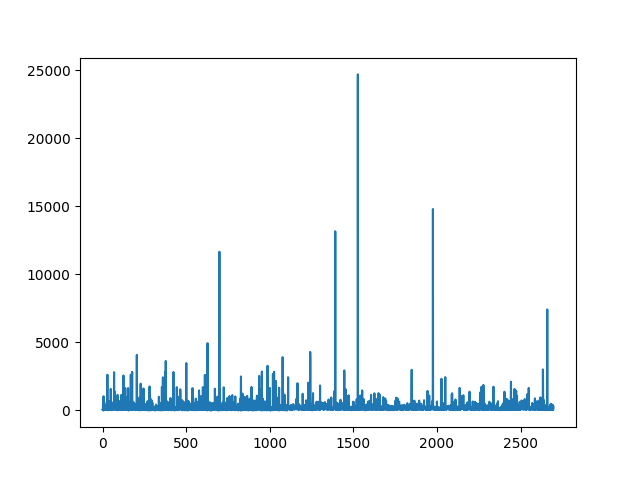
\includegraphics[width=1\textwidth]{SHtailleMail}
\caption{liste des tailles des mails}
\centering
\end{figure}
Il n’est pas possible de considérer tous les cas possibles car il y a trop de tailles différentes (elles varient de 2 à 25 000): le modèle serait trop compliqué à entraîner.
\begin{figure}[H]
\includegraphics[width=1\textwidth]{SHhisttailles}
\caption{Histogramme de la taille des mails de moins de 5000 mots}
\centering
{\footnotesize L'histogramme est inexploitable car les valeurs ne sont pas bien réparties.\par}
\end{figure}
\end{minipage}


\begin{minipage}{\textwidth}
Afin d'égaliser l'histogramme, nous avons choisi de travailler avec le logarithme de la taille des mails.
\begin{figure}[H]
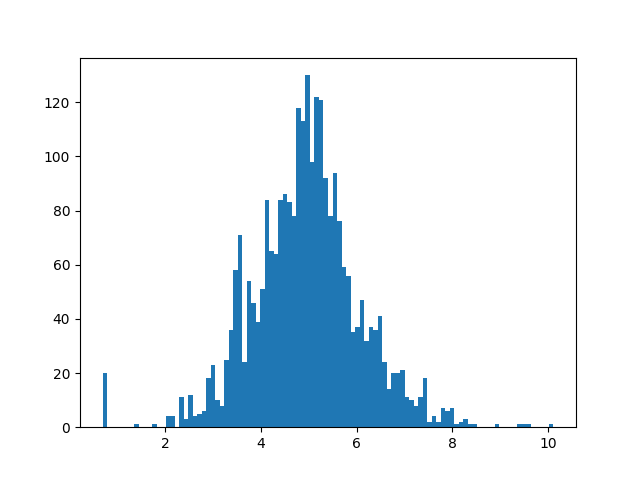
\includegraphics[width=1\textwidth]{SHlog100}
\caption{histogramme du log des tailles (avec 100 catégories)}
\end{figure}
Les valeurs de l'histogramme sont mieux réparties. Cependant, les bornes extérieures de l'histogramme sont trop dispersées pour servir à quelque chose.
\end{minipage}

\begin{minipage}{\textwidth}
Nous avons choisi de ramener les abscisses de l'histogramme précédent dans l'intervalle \text{[2,8]}.\\ Note : cela revient à considérer les mails contenant moins de $e^2\approx 8$ mots comme faisant 8 mots de long et de même pour les mails de plus de $e^8\approx 2980$ mots.
\begin{figure}[H]
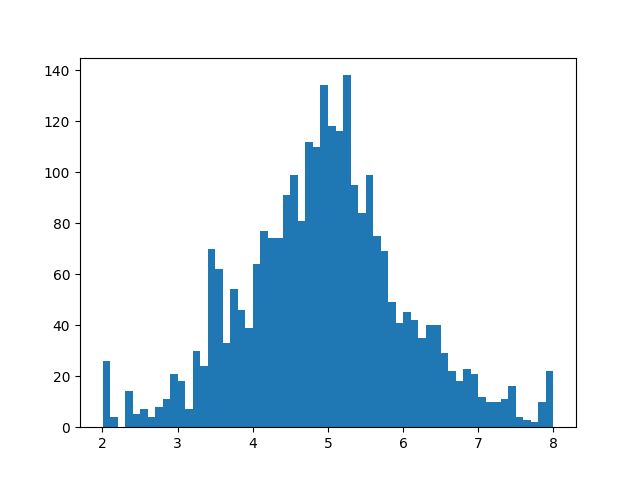
\includegraphics[width=1\textwidth]{SHlog10}
\caption{histogramme du log ramené en [2,8] (60 catégories)}
\end{figure}
\end{minipage}

\begin{minipage}{\textwidth}
Les 60 catégories de l'histogramme précédent ne sont pas représentatives. De plus, lors de l'apprentissage, les hams sont séparés des spams, la taille de l'instance d'apprentissage est donc deux fois plus petite et les valeurs sont donc moins précises. Nous avons donc décidé de ne garder que 24 catégories. Finalement, pour l'affichage comme pour les calculs, nous utilisons la proportion plutôt que le nombre de mails.
\begin{figure}[H]
\centering
{\footnotesize a) Apprentissage sur la liste des hams\par}
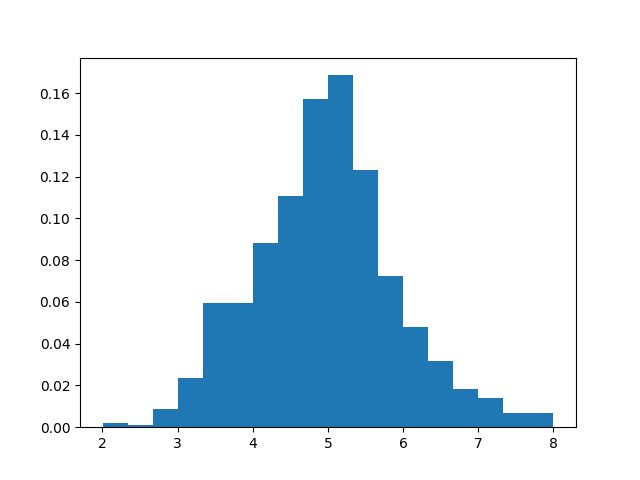
\includegraphics[width=1\textwidth]{Hlog3P}
{\footnotesize \\b) Apprentissage sur la liste des spams\par}
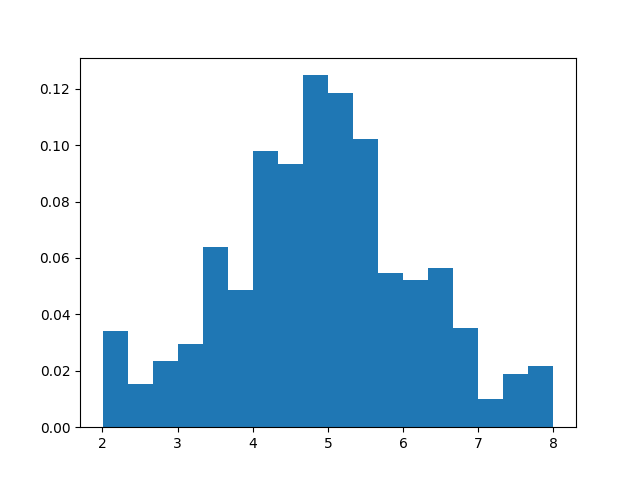
\includegraphics[width=1\textwidth]{Slog3P}
\caption{histogrammes du log, ramenés en [2, 8], avec 24 catégories}
\end{figure}
\end{minipage}

\subsection{}
Voir le code ainsi que la partie  \ref{partie2.1}

\subsection{}
\begin{minipage}{\textwidth}
Avec f(x) le résultat de la fonction predit-email pour un mail de taille x, on a :\\
P(f(x) = 1 | Y = -1): probabilité que le mail soit détecté comme spam alors qu'il n'en est pas (c'est un "faux-positif").\\
P(f(x) = -1 | Y = 1): probabilité que le mail ne soit pas détecté comme spam alors qu'il l'est (c'est un "faux-négatif"). Notons que cette erreur est beaucoup moins grave que la précédente.\\
Avec la liste de spam fournie, il y a 63\% de faux-négatifs. C'est à dire que presque deux spams sur trois seraient conservés.\\
Avec la liste de ham fournie, il y a 32\% de faux-positifs. C'est à dire qu'environ un vrai message sur trois serait supprimé.\\
En moyenne, on obtient 44\% d'erreur.\\\\
En séparant la liste d'apprentissage et la liste de test, en faisant varier le pourcentage pris pour l'apprentissage, on obtient :
\[\begin{array}{cccc}
pourcentage & faux\text{-négatifs} & faux\text{-positifs} & moyenne\\
10 & 51\% & 44\% & 47\%\\
20 & 71\% & 18\% & 40\%\\
30 & 71\% & 27\% & 45\%\\
40 & 65\% & 30\% & 45\%\\
50 & 63\% & 32\% & 45\%\\
60 & 63\% & 33\% & 45\%\\
70 & 65\% & 31\% & 45\%\\
80 & 61\% & 33\% & 44\%\\
90 & 64\% & 32\% & 45\%
\end{array}\]

Les taux de faux-positifs et faux-négatifs fluctuent légèrement mais la moyenne d'erreur reste aux alentours de 44\%. Sans classifieur, nous aurions 50\% d'erreurs. La conclusion est que \textbf{ce classifieur est presque inutile}.
\end{minipage}

\newpage
\section{Classification à partir du contenu d'un e-mail}
\subsection{}
Il n'est pas raisonnable de calculer la distribution P(X = x | Y = 1) car P(X = x) est la probabilité qu'un mail contienne exactement une liste de mot. Cet événement est beaucoup trop précis et sa probabilité associée serait presque nulle. Avec 1000 mots dans le dictionnaire, on aurait $2^{1000}$ événements.\\
En réalité, l'hypothèse d'indépendance entre les mots n'est pas respectée, par exemple si un verbe conjugué apparaît, il y a de plus fortes chances que le sujet qui lui correspond apparaisse.

\subsection{}
\begin{minipage}{\textwidth}
\begin{figure}[H]
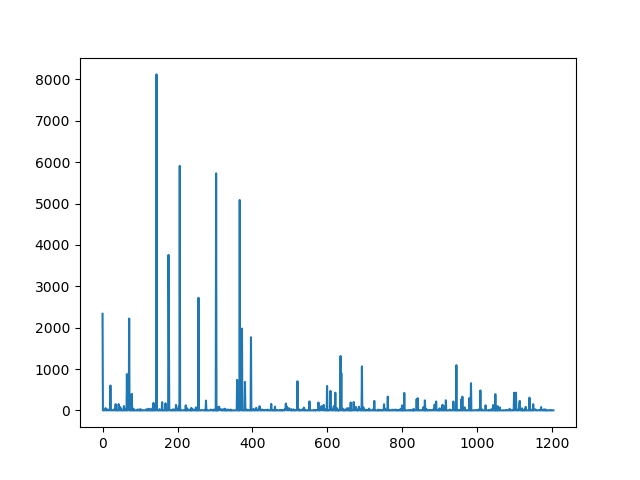
\includegraphics[width=1\textwidth]{apparitionmot}
\caption{histogramme du nombre d'apparition des 50 premiers hams et spams}
Note : la hauteur de la première barre est d'environ 5000
\end{figure}

Afin d'interpréter plus facilement les mails, on convertit tous les mails en minuscule. Les mails fournis étant en anglais, il n'y a pas de problèmes d'accent. La ponctuation est aussi filtrée lorsque l'on récupère les mots des mails. Finalement, on a utilisé un "stemmer" qui simplifie les mots.\\
La grande majorité des mots n'apparaît qu'une fois, il est inutile de les ajouter au dictionnaire. Plus généralement, les mots n'apparaissant que peu de fois risquent d'être peu utilisés lors des tests et de ne pas être fiables.\\
Les mots apparaissant à peu près autant de fois dans les spams et dans les hams ne nous donnent pas beaucoup d'information non plus. Nous conserverons en priorité les mails qui penchent fortement vers une catégorie.\\
\end{minipage}

\subsection{}
\begin{minipage}{\textwidth}
La méthode utilisée programmer et tester le classifieur est la suivante :\\
1- Récupérer les mots des mails en minuscule et les simplifier grâce à un stemmer.\\
2- Séparer la liste des mails en 75\% pour l'apprentissage et les 25\% restants pour les tests.\\
3- Créer le dictionnaire et ne garder que les mots apparaissant suffisamment de fois.\\
4- Trier les mots du dictionnaire en mettant en premier les mots qui penchent fortement d'un côté.\\
5- Ne garder que les n premiers mots.\\
6- calculer taux erreur sur les mails restants.\\
7- Boucler 30 fois à l'étape 2.\\
\\
Durant les tests, nous avons remarqué que lorsque l'on ne compte garder qu'un nombre fixé de mails, fixer une valeur minimale d’occurrence des mots avait très peu d'impact, de même que l'utilisation du stemmer.\\

Concernant les graphiques ci-dessous:\\
- Nous avons fait varier la taille maximale du dictionnaire aux puissances de 2 allant de $2^2=4$ à $2^{16}=65536$. La longueur du dictionnaire est toujours égale à la taille maximale autorisée, sauf pour la dernière catégorie où les données d'apprentissage ne fournissent pas assez de mots (la taille du dictionnaire est alors de 50 000 mots environ).\\
- L'axe des abscisses représente le log en base 2 de la taille maximale du dictionnaire.\\
- Pour une taille donnée, les points bleus représentent la performance des 30 tests.\\
- La ligne orange passe par les moyennes des tests.

\begin{figure}[H]
\includegraphics[width=1\textwidth]{16log30testtoken1occ}
\caption{apprentissage sur 75\%}
\end{figure}
\end{minipage}

\begin{minipage}{\textwidth}
\begin{figure}[H]
\includegraphics[width=1\textwidth]{16log30testtoken51occ}
\caption{apprentissage sur 75\% avec 51 occurrences minimum}
\end{figure}
Bien qu'imposer un nombre minimal d'occurrence change le dictionnaire, les résultats obtenus sont similaires. Sans limite de taille, avec un nombre d'occurrence minimal à 2, on divise la taille du dictionnaire par 3 sans changer ses performances.

\[\begin{array}{ccccc}
\text{occurrences minimales} & \text{Taille moyenne du dictionnaire} & spam & ham & moyenne\\
1 & \text{36450 mots} & 6,2\% & 4,0\% & 4,9\%\\
2 & \text{13080 mots} & 6,5\% & 4,2\% & 5,2\%
\end{array}\]
Ces taux d'erreur ont été obtenu en faisant la moyenne des résultats sur 100 expériences.\\\\

A partir de 50 occurrences, une perte de précision commence à être visible.
\end{minipage}

\begin{minipage}{\textwidth}
\begin{figure}[H]
\includegraphics[width=1\textwidth]{16log30testtoken1occ90pour}
\caption{apprentissage sur 90\%}
\end{figure}
Augmenter la taille des données d'apprentissage réduit la taille des tests, ce qui augmente l'écart type des valeurs mesurées. Les performances des petits dictionnaires semblent s'améliorer légèrement (passage de 16\% à 15\% d'erreur pour un dictionnaire de 64 mots par exemple).

\end{minipage}



\section{Conclusion}
Classifier les mails selon leur taille ne fonctionne pas, le taux d'erreur obtenu étant de 44\%.

La classification par mot est d'une efficacité surprenante, les meilleurs taux obtenus étant de l'ordre de 5\% d'erreur. Comme on pouvait s'y attendre, plus la taille du dictionnaire est grande et plus le temps de calcul augmente, mais les performances du classifieur augmentent aussi. On retiendra qu'on peut au moins réduire la taille du dictionnaire d'un facteur 4 sans perdre de précision. Les résultats obtenus étaient de l'ordre de 6\% d'erreur sur les spams et de 4\% sur les hams, on pourrait chercher à diminuer encore le taux d'erreur sur les hams, quitte à l'augmenter sur les spams.

Les classifieurs utilisés par nos boîtes mail sont encore plus performants. Une possibilité pour améliorer les performances de notre classifieur serait de ne pas séparer les groupes de mots d'une phrase.


\end{document}
